\documentclass[12pt]{article}

\usepackage{geometry}
\usepackage{amsmath,amsthm,amssymb}
\usepackage{graphicx}
\usepackage{multicol}

\newcommand{\lemma}{\noindent \textbf{Lemma: }}
\newcommand{\thm}{\noindent \textbf{Theorem: }}
\newcommand{\lskip}{\vspace{\baselineskip}}

\begin{document}

\title{AVL Trees}
\author{}
\maketitle

\section*{Description}
AVL trees are self-balancing BSTs that are strictly balanced. The invariant of an AVL tree is that for any node in the tree, the height of the left child and the height of the right child differ by at most 1. This invariant is maintained through rotations after insertion and deletion.

\section*{Insertion}
The first part of insertion is the same as inserting into a regular BST. However, inserting may cause one or more nodes in the tree to become imbalanced. Note that when we insert a value, the only nodes whose heights change are the ancestors of the node that we inserted. So, if inserting a node causes imbalance, the inserted value must have at least two ancestors (otherwise the length of the path from the root to the inserted node has increased to at most 1, which cannot cause an imbalance since this would require a height of -1 in the other subtree).

Now, suppose that inserting a node $v$ caused an imbalance. Let $z$ be the first node on the path from $v$ to the root that was imbalanced. Let $y$ be the child of $z$ on that path and $x$ be the grandchild of $z$ on that path. Since $z$ became imbalanced, we know the $h(y)$ increased and therefore the $h(x)$ increased as well. Suppose originally $h(x) = m$. There are 4 cases:

\begin{enumerate}
  \item LL: $y$ is the left child of $z$ and $x$ is the left child of $y$.

  \begin{figure}[!ht]
    \centering
    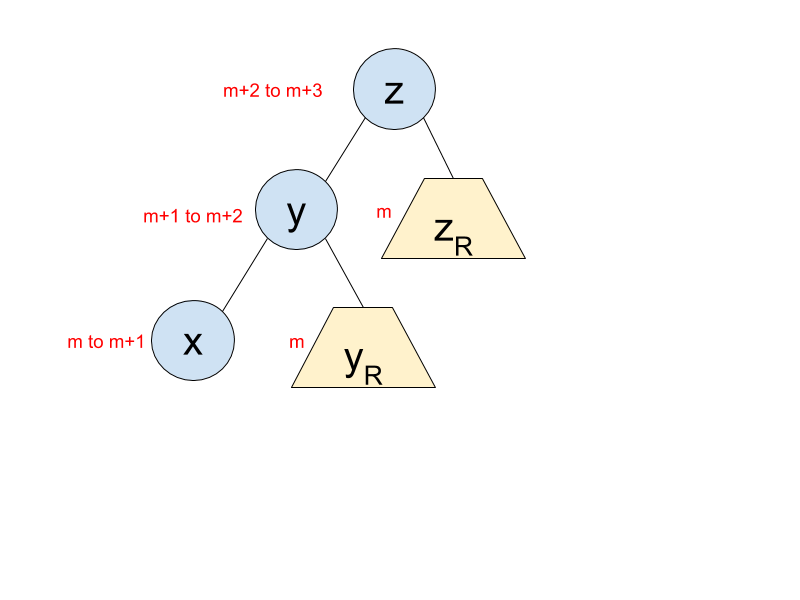
\includegraphics[trim=50 50 150 40, clip,scale=0.33]{pics/avl_tree/insert_ll1}
    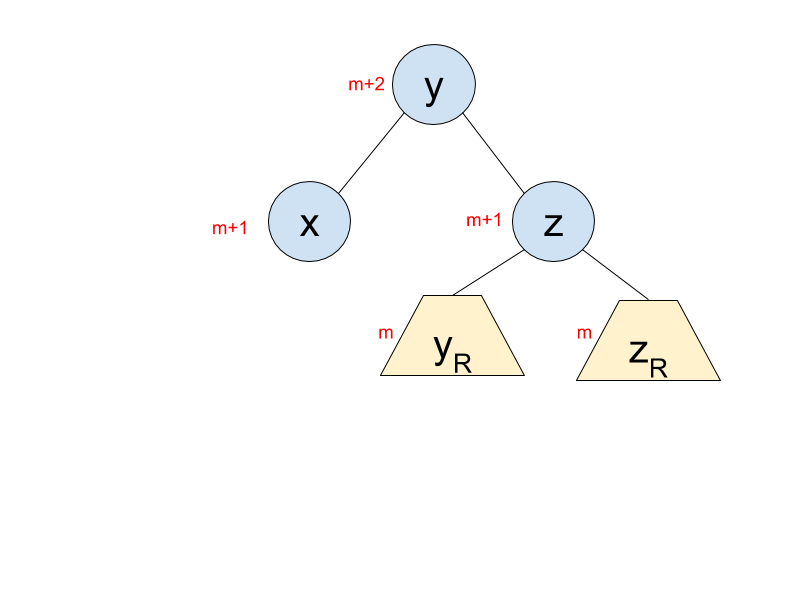
\includegraphics[trim=250 50 50 40, clip,scale=0.33]{pics/avl_tree/insert_ll2}
    \caption{LL rotation on insertion}
  \end{figure}

  Since $h(x)$ was $m$, that means $h(y_R)$ be $m-1, m$, or $m+1$, since $y$ was balanced. After the insertion $h(x) = m+1$. Now, $y$ is still balanced, so $h(y_R) \neq m-1$. Since $h(y)$ increased, $h(y_R) \neq m+1$. Therefore, $h(y_R) = m$. Thus, $h(y)$ increased from $m+1$ to $m+2$.

  Now, since the $h(y)$ was $m+1$, $h(z_R)$ could be $m, m+1$, or $m+2$. Since $z$ is now imbalanced, we know $h(z_R) = m$. Therefore, $h(z)$ increased from $m+2$ to $m+3$. After the rotation, we can see that all the nodes are balanced. Also note that the height of the subtree is $m+2$ both before the insertion and after the rotation. This means that since all ancestors of this node were balanced before the insertion, they will all be balanced again after the rotation. Therefore, when inserting, we do not need to check any ancestor nodes after the initial rotation.

  \item RR: $y$ is the right child of $z$ and $x$ is the right child of $y$. This is analogous to the previous case.

  \item LR: $y$ is the left child of $z$ and $x$ is the right child of $y$.

  \begin{figure}[!ht]
  \centering
    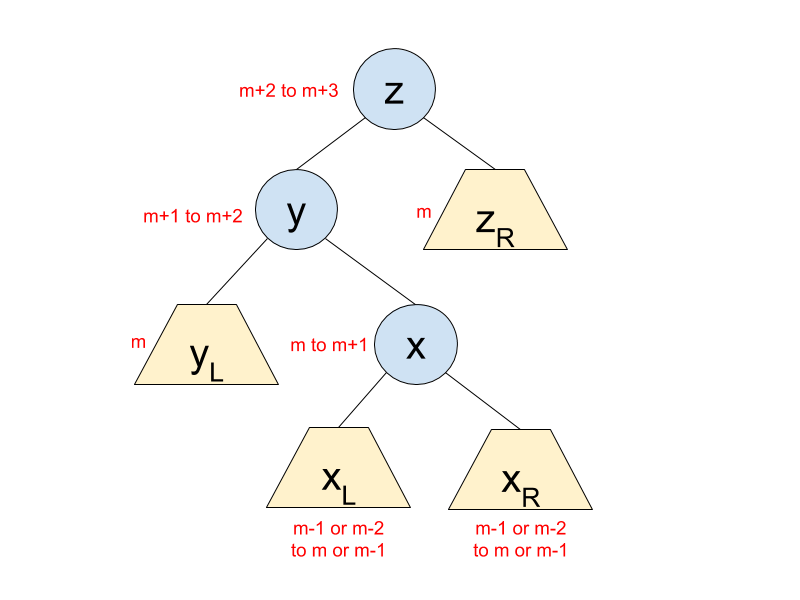
\includegraphics[trim=50 0 150 40, clip,scale=0.33]{pics/avl_tree/insert_lr1}\\
    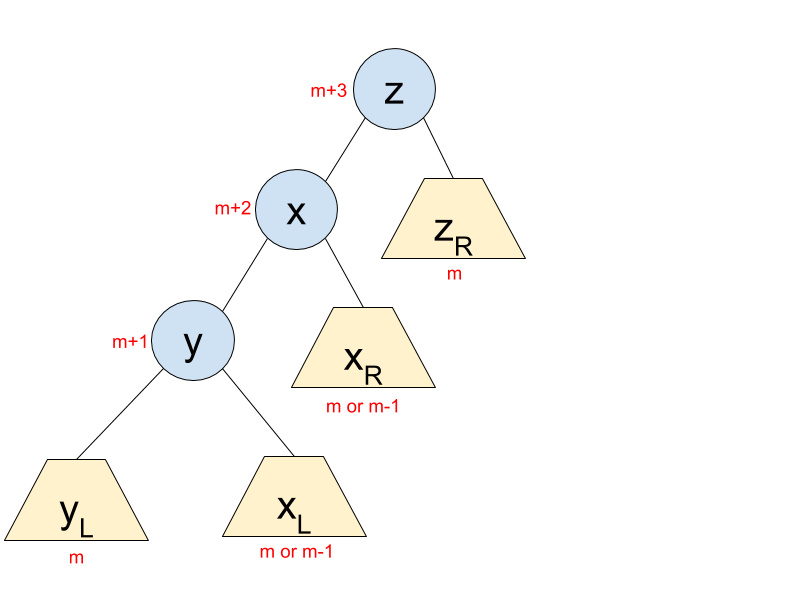
\includegraphics[trim=0 0 250 40, clip,scale=0.33]{pics/avl_tree/insert_lr2}
    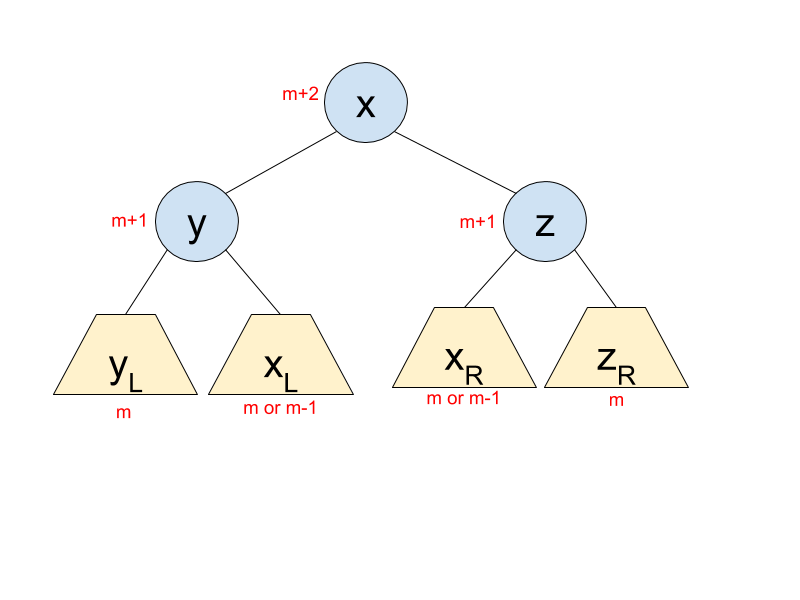
\includegraphics[trim=50 50 50 40, clip,scale=0.33]{pics/avl_tree/insert_lr3}
    \caption{LR rotation on insertion}
  \end{figure}

  Since $h(x)$ was $m$, that means $h(y_L)$ can be $m-1, m$, or $m+1$, since $y$ was balanced. After the insertion $h(x) = m+1$. Now, $y$ is still balanced, so $h(y_L) \neq m-1$. Since $h(y)$ increased, $h(y_L) \neq m+1$. Therefore, $h(y_L) = m$. Thus, $h(y)$ increased from $m+1$ to $m+2$.

  Now, since the $h(y)$ was $m+1$, $h(z_R)$ could be $m, m+1$, or $m+2$. Since $z$ is now imbalanced, we know $h(z_R) = m$. Therefore, $h(z)$ increased from $m+2$ to $m+3$.

  Since $h(x)$ was $m$, that means one of $h(x_L)$ and $h(x_R)$ was $m-1$ before the insertion and the other was $m-1$ or $m-2$. After the insertion, $x$ is still balanced, so one of them is $m$ and the other is $m$ or $m-1$. (We can actually show that they must both be $m-1$ before, but it is not important for this proof.)

  After the double rotation, we can see that all the nodes are balanced. Also note that the height of the subtree is $m+2$ both before the insertion and after the rotation, which implies the same as before.

  \item RL: $y$ is the right child of $z$ and $x$ is the left child of $y$. This is analogous to the previous case.

\end{enumerate}

\section*{Deletion}
The first part of deletion is the same as deleting from a regular BST. However, deletion may cause one or more nodes in the tree to become imbalanced. Let $z$ be the first imbalanced ancestor of the deleted node. Again, $z$ must have a height of at least 2 to have an imbalance. Let $y$ be the child of $z$ of greater height and $x$ be the child of $y$ with greater height (the left one if they are equal). Note that since $z$ became imbalanced, $y$ cannot be in the subtree we just deleted from. There are 4 cases:

\begin{enumerate}
  \item LL: $y$ is the left child of $z$ and $x$ is the left child of $y$.

  \begin{figure}[!ht]
    \centering
    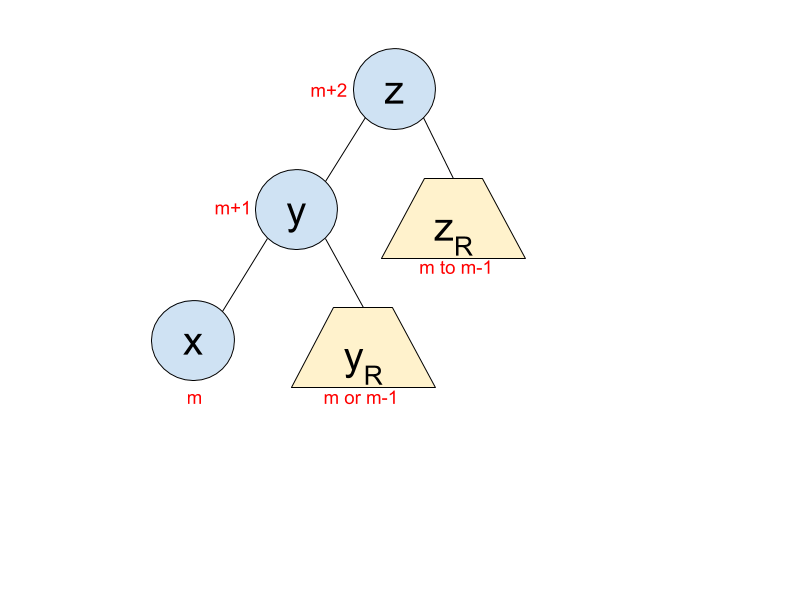
\includegraphics[trim=50 50 150 40, clip,scale=0.33]{pics/avl_tree/delete_ll1}
    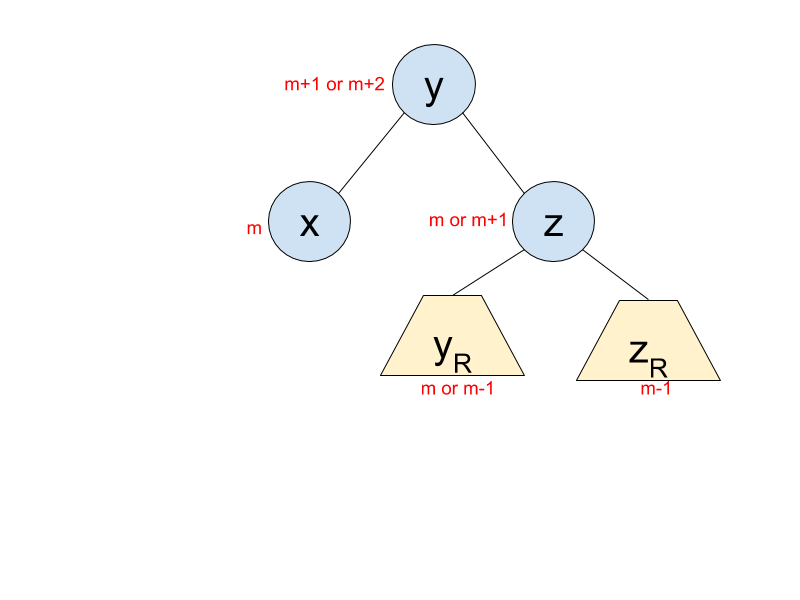
\includegraphics[trim=250 50 50 40, clip,scale=0.33]{pics/avl_tree/delete_ll2}
    \caption{LL rotation on deletion}
  \end{figure}

  Suppose $h(z_R) = m$ before the deletion. Since $z$ became imbalanced, $h(z_R)$ must have decreased as a result of the deletion, so $h(z_R) = m-1$ after. Also since $z$ became imbalanced, $h(y) = m+1$. We know $h(x) \geq h(y_R)$, so since $y$ is balanced, $h(x) = m$ and $h(y_R) = m$ or $m-1$.

  After the rotation, we can see that all the nodes are balanced. However, note that the height of the subtree may have changed from $m+2$ to $m+1$ from before the deletion to after the rotation. This means one of $z$'s ancestors may have become imbalanced. Unlike insertion, we must check all the ancestors and balance them if necessary.



  \item RR: $y$ is the right child of $z$ and $x$ is the right child of $y$. This is analogous to the previous case.

  \item LR: $y$ is the left child of $z$ and $x$ is the right child of $y$.

  Suppose $h(z_R) = m$ before the deletion. By the same logic as in the first case, we have $h(z_R) = m-1$ after the deletion and $h(y) = m+1$. We know $h(x) > h(y_L)$, so since $y$ is balanced, $h(x) = m$ and $h(y_L) = m-1$. Since $x$ is balanced, $h(x_L)$ and $h(x_R)$ are $m-1$ or $m-2$.

  After the rotation, we can see that all the nodes are balanced, but again, the height of the subtree has changed, so we must check all the ancestors.

  \begin{figure}[!ht]
  \centering
    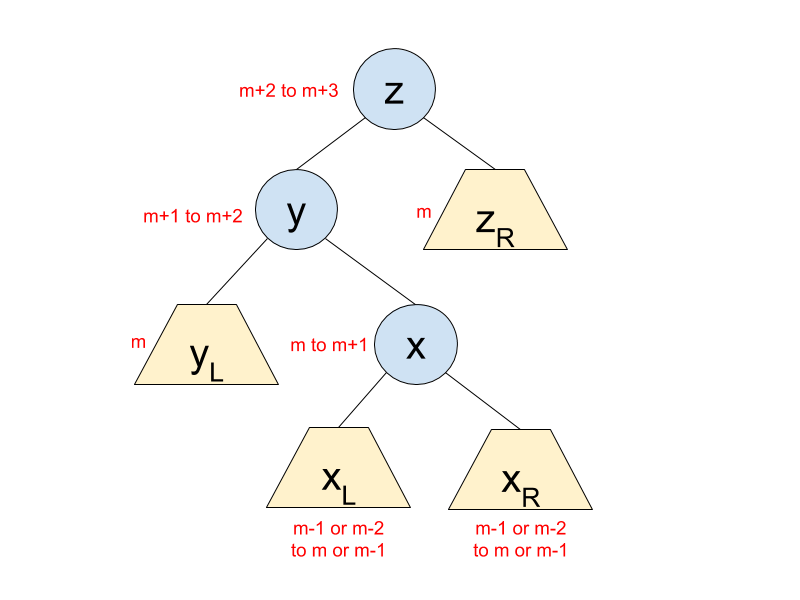
\includegraphics[trim=50 0 150 40, clip,scale=0.33]{pics/avl_tree/insert_lr1}\\
    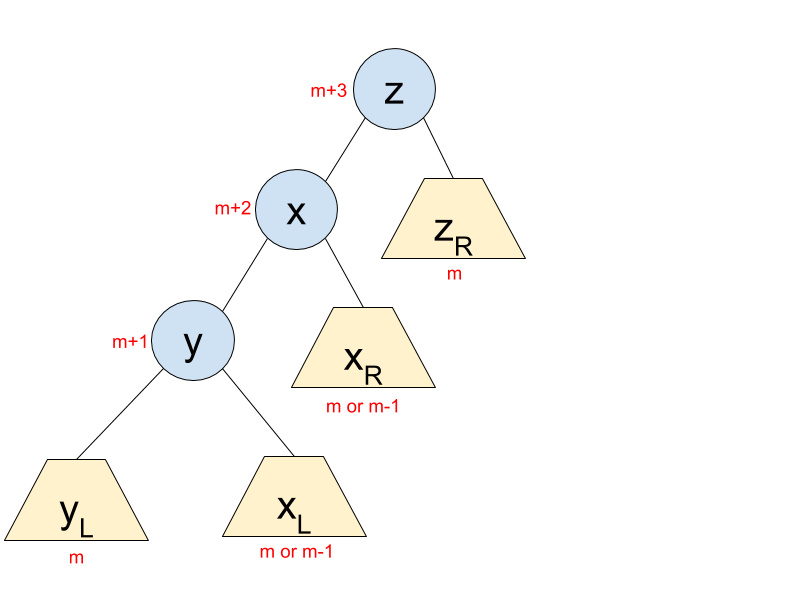
\includegraphics[trim=0 0 250 40, clip,scale=0.33]{pics/avl_tree/insert_lr2}
    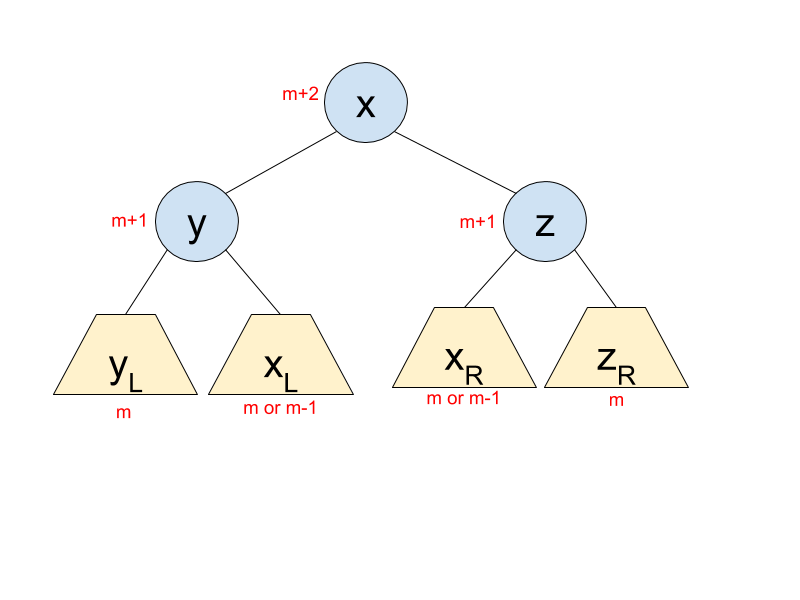
\includegraphics[trim=50 50 50 40, clip,scale=0.33]{pics/avl_tree/insert_lr3}
    \caption{LR rotation on deletion}
  \end{figure}

  \item RL: $y$ is the right child of $z$ and $x$ is the left child of $y$. This is analogous to the previous case.

\end{enumerate}

\section*{Time Complexity}
Given a height $h$, let $T_h$ be the AVL tree with the fewest possible number of nodes. Since $h$ is the asymptotic time it takes for each one of an AVL tree's methods, $T_h$ has the worst possible runtimes as a function of the number of nodes. We can see that $T_0 = 0$ and $T_1 = 1$, and in general $T_h$ has a root with $T_{h-1}$ and $T_{h-2}$ as subtrees.
\begin{figure}[h]
  \centering
  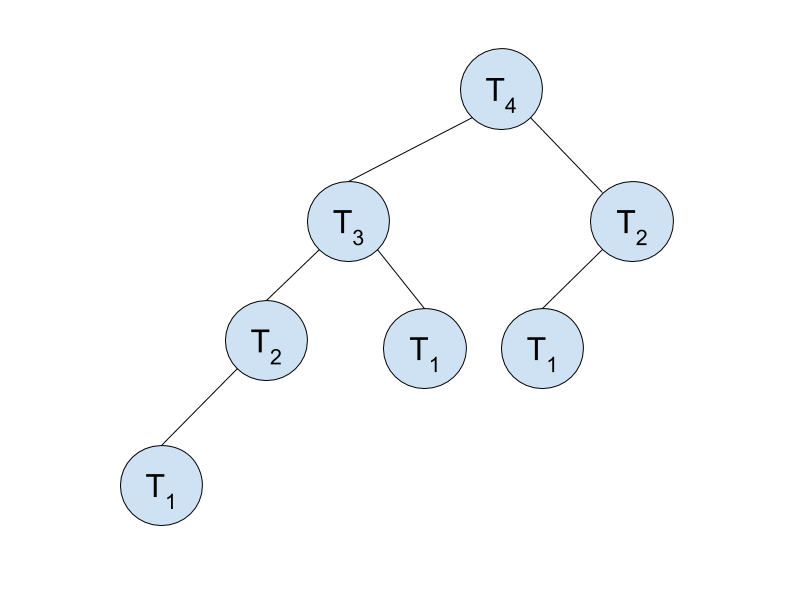
\includegraphics[scale=0.5]{pics/avl_tree/time_comp} \\
  \caption{Worst-case AVL tree of height 4}
\end{figure}

Letting $N_h$ be the number of nodes in $T_h$, we have $N_h = N_{h-1} + N_{h-2} + 1$. Solving the recurrence relations yields $N_h = \frac{1}{2}\left(3F_h + L_h + 2\right)$, where $F_h$ and $L_h$ are the $h^{th}$ Fibonacci and Lucas numbers, respectively. We know $F_n = \frac{1}{\sqrt{5}}\left( \phi^n - \overline{\phi}^n \right)$ and $L_n = \phi^n + \overline{\phi}^n $, where $\phi$ is the golden ratio and $\overline{\phi} = 1 - \phi$. Therefore, $N_h \in O(\phi^h)$. So, our worst case runtime on an AVL tree of height $h$ occurs when the tree has about $\phi^h$ nodes. So, the runtime is $O(h) = O(\log_{\phi}n)$.
We can see that $\log_{\phi}n = \frac{\log_2 n}{\log_2 \phi} \approx 1.44 \log_2 n$, so the worst-case AVL lookup time is about 1.44 times worse than a perfectly balanced tree.




\end{document}
